\documentclass{standalone}
\usepackage{pgfplots}
\newcommand{\point}[2]{\pgfextractx{\dimen0}{\pgfpointanchor{#1}{#2}}\pgfextracty{\dimen2}{\pgfpointanchor{#1}{#2}}\typeout{POINT #1.#2: \the\dimen0,\the\dimen2}}
\begin{document}
\begin{tikzpicture}
\begin{axis}[axis x line=middle,axis y line=middle,
  xmin=-2,xmax=-1,ymin=-4,ymax=-3,enlargelimits=true]
\end{axis}
\typeout{CASE negative}
\point{current axis}{south west}\point{current axis}{north east}\point{current axis}{origin}
\end{tikzpicture}
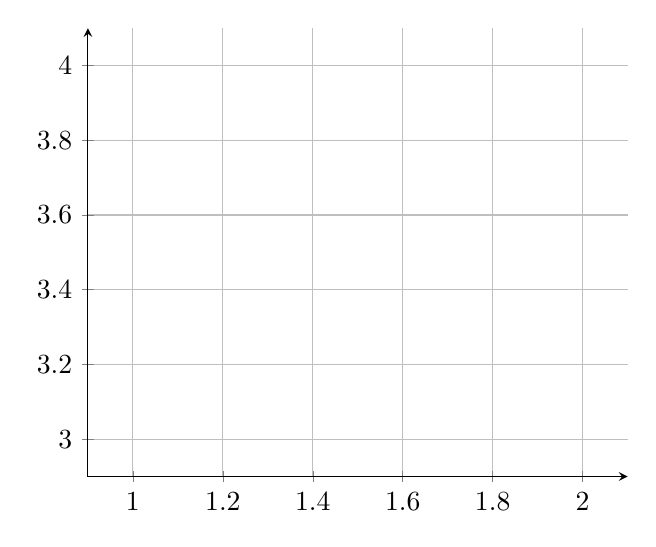
\begin{tikzpicture}
\begin{axis}[axis x line=middle,axis y line=middle,
  xmin=1,xmax=2,ymin=3,ymax=4,enlargelimits=true,grid=major]
\end{axis}
\typeout{CASE positive}
\point{current axis}{south west}\point{current axis}{north east}\point{current axis}{origin}
\end{tikzpicture}
\end{document}
